\documentclass{hippoidC}
% \frontmatter
\newcommand{\obc}{\text{ob}\thinspace\mathcal{C}}
\usepackage{float}
\usepackage{standalone}
\usepackage{tikz}
\usepackage{tikzit}
\usepackage{titlesec}
\usepackage{tocloft} % Provides ToC customization


\input{sample-02.tikzstyles}

% \memoto{Idris}
% \memosubject{Joy of Abstraction}
% \memodate{2024.03.26}
\newenvironment{proofitem}
{ \begin{itemize}[label={}, leftmargin=2mm, itemsep=0.5mm] }
{\end{itemize}}

\newcounter{tttacounter}
\counterwithin{tttacounter}{section} % Question counter resets with each section
\newenvironment{ttta}{
    \par\vspace{0.5cm}
    \noindent\hrulefill
    \par\vspace{0.2cm}
    \stepcounter{tttacounter} % Increment the counter
    \textbf{\textsc{TTTA} \thetttacounter{}} % Display the counter
    \ignorespaces
    \addcontentsline{toc}{subsubsection}{\textsc{T} \thetttacounter} % Add to ToC
}
{\par\vspace{0.0cm}}

\theoremstyle{definition}
\newtheorem{definition}{Definition}[subsection] % Can be changed to other levels

% \includeonly{set theory}

\begin{document}
\large
% \include{title}
\tableofcontents
% \mainmatter
\setcounter{section}{7}
\section{Categories, the Definition}
\begin{definition}
    The data in a category consists of objects and arrows.
    \begin{enumerate}
    \item Objects: a collection $\obc{}$ of objects
        \item Arrows: for objects $a, b\in \obc{}$, a collection
        $\mathcal{C}(a, b)$ of arrows $f: a\rightarrow b$. These arrows are not
        limited to functions, even though we use function notation to denote
        them;
    \end{enumerate}
\end{definition}
\begin{definition}
The structure in a category consists of identities and composition.
\begin{align*}
1_a : a \rightarrow a&&\text{identity}\\
f: a\rightarrow b&&\text{composition}\\
g: b\rightarrow c\\
g\circ f: a\rightarrow c
\end{align*}
\end{definition}
\begin{definition}
The properties in a category consists of unitality and associativity.
\begin{align*}
f: a\rightarrow b\\
f\circ 1_a = f = 1_b \circ f\\
    f:& a\rightarrow b\\
    g:& b\rightarrow c\\
    h:& c\rightarrow d\\
    (h\circ g)\circ f=&h\circ (g \circ f)
\end{align*}
\end{definition}
For a category to really be a category, there are seemingly four requirements:
identity arrows, composition, unitality, and associativity. But notice that the
unitality property requires identity arrows, and the associativity property
requires composition. So there are two properties, and both will fail if the
precondition is not met.

\section{Examples previously seen in book}
\subsection{Equivalence Relation as a Category}
\begin{proofitem}
    \item
\begin{align}
    x \in S \implies (x, x) \in S &&\text{reflexivity}\\
    (x,y) \in R \implies (y, x) \in R &&\text{symmetry}\\
    (x,y) \land (y, z) \in R \implies (x, z) \in R &&\text{transitivity}
\end{align}
\item
Categories can be seen to be inspired by equivalence relations. Start with a set
$S$ that has an equivalence relation $R$.
\begin{enumerate}
    \item Objects: $x\in S$.
    \item Arrows: $x\in R\subseteq S\times S$.
\end{enumerate}
\item Let $\mathcal{C}_{\text{eq}}$ be the category formed from an equivalence
    relation.
\item To show that $R$ and $S$ form a category, we must show that it adheres to
    the two required properties of categories: unit laws and associativity.
\item The unit laws requires that for any arrow $f:a \rightarrow b$, there
    exists arrows $1_a \land 1_b$ such $f\circ 1_a = f = 1_b \circ f$.
\begin{figure}[H]
\begin{align*}
    f\circ 1_a=& (a, b)\circ (a, a)&\exists(a,a)\text{ from reflexivity}\\
    =&(a, b)\\
    =&f\\
    1_b\circ f=& (b, b)\circ (a, b) &\exists(b,b)\text{ from reflexivity}\\
    =&(a, b)\\
    =&f
\end{align*}
\caption{Unital Laws}
\end{figure}
\item Thus we have shown the category $\mathcal{C}_{\text{eq}}$ adheres to the unital laws.
\item The associativity laws requires that for arrows $f, g, h,
        a \overset{f}{\rightarrow} b \overset{g}{\rightarrow} c
        \overset{h}{\rightarrow} d, (h\circ g)\circ f=h\circ (g \circ f)$.
\begin{figure}[H]
\begin{align*}
    (h\circ g)\circ f=&((c, d)\circ (b, c))\circ (a, b)\\
    =&(b, d)\circ (a, b)&\text{via transitivity}\\
    =&(a, d)\\
    h\circ (g\circ f)=&(c, d)\circ ((b, c))\circ (a, b))\\
    =&(c, d)\circ (a, c)&\text{via transitivity}\\
    =&(a, d)
\end{align*}
\caption{Associative Laws}
\end{figure}
\item Thus we have shown the category $\mathcal{C}_{\text{eq}}$ adheres to the
    associative laws.
\item Conversely, can you put some conditions on a category to ensure that it
    “is” an equivalence relation?
\item To assure that some category $\mathcal{C}$ forms an equivalence relation,
    we must assure that that $\mathcal{C}$ gives rise to three properties
    required for an equivalence relation: reflexivity, symmetry, and
    transitivity. Reflexivity and transitivity are guaranteed for any category
    via the unital and associative properties---requirements to be a category. To
    satisfy symmetry, for any arrow $f:a\rightarrow b\in \mathcal{C}$, there
    must exist an arrow $g:b\rightarrow a\in \mathcal{C}$.

    Additionally, there can be only arrow between any two objects $a, b \in
    \mathcal{C}$. This uniqueness property between two objects is required
    because a relation $R$ is a set, and a set is defined by some characteristic
    function, which is a function with a boolean codomain. Either an element is
    in or out of the set, and more than one arrow between the same objects would
    violate this requirement.
\end{proofitem}

\begin{table}
    \centering % Optional, for centering the table
    \begin{tabular}{ ccccc } % 5 columns, each centered
    \hline
    & Equivalence Relation & & Category & \\ \hline
    Data & objects & $\rightarrow$ & objects& Data\\
    Structure & relations & $\rightarrow$ & arrows & \\ \hline
    & reflexivity & $\rightarrow$ & identities & \\
    Properties & symmetry & $\rightarrow$ & inverses & Structure \\
    & transitivity & $\rightarrow$ & composition & \\\hline
    & & & unit laws& Properties \\
    & & & associativity &
    \\\hline
    \end{tabular}
    \caption{Properties become structure, and a new layer of properties is required.}
\end{table}
\subsection{Factors of $n\in\mathbb{N}$ as a Category}
Pick a number. The objects are the factors, and the arrows $a\rightarrow b$ are
whenever a is a factor of $b$. In this cateogry, like the equivalence-relation
category, there is at most one arrow between two objects. That is because this
category is again representing a relation. Any relation $(a, b)$ can only be in
a set once, per the definition of set.
\begin{figure}[H]
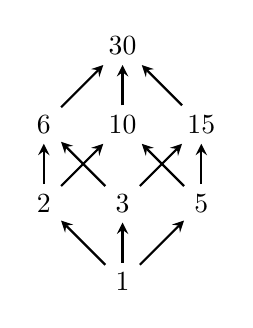
\begin{tikzpicture}[->, >=stealth, thick]
\node (1) at (2,0) {$1$};
\node (2) at (1,1) {$2$};
\node (3) at (2,1) {$3$};
\node (5) at (3,1) {$5$};
\node (6) at (1,2) {$6$};
\node (10) at (2,2) {$10$};
\node (15) at (3,2) {$15$};
\node (30) at (2,3) {$30$};
\draw (1) -- (2);
\draw (1) -- (3);
\draw (1) -- (5);
\draw (2) -- (6);
\draw (2) -- (10);
\draw (3) -- (6);
\draw (3) -- (15);
\draw (5) -- (10);
\draw (5) -- (15);
\draw (6) -- (30);
\draw (10) -- (30);
\draw (15) -- (30);
\end{tikzpicture}
\caption{30-factor Category}
\end{figure}
\subsection{Factors of $\mathbb{N}$ as a Category}
If we took all of $\mathbb{N}$ as a category, then there would be a morphism
from $0$ to all other objects, except itself. In fact, $0$ couldn't be in the
category, because there couldn't be an identity relation as $\frac{0}{0}$ is
undefined. If we modify the set to be $\mathbb{N} - \set{0}$, then there would
be a morphism from $1$ to all other elements. Each prime number would have two
morphisms---the identity morphism and one from $1$ to itself.

\section{Ordered Sets}
\begin{definition}
A totally ordered set is a set $S$ plus a relation $R$ on the set (called a total
order) that satisfies the conditions for a partial order plus an additional
condition known as the comparability condition. A relation $\geq$ is a total order
on a set $S$ ($\geq$ totally orders $S$) if the following properties hold.
\setcounter{equation}{0}
\begin{align}
    a\leq a, \forall a \in S&&\text{reflexive}\\
    a\leq b \land b\leq a \implies a=b&&\text{antisymmetric}\\
    a\leq b \land b\leq c \implies a\leq c&&\text{transitive}\\
    \forall a,b \in S, a\leq b \lor b\leq a&&\text{trichotomy}
\end{align}
\end{definition}
\subsection{Totally Ordered Set}
A totally ordered set defines a category $\mathcal{C}$ where $\forall a, b \in
\obc{}$, there is exactly one arrow between them.
\begin{ttta}
Let's check if this is true for the category of $\mathbb{N}$ with the relation $\geq$.
\end{ttta}
\begin{proofitem}
\item Let $T$ be a totally ordered set.
\item Let $R\subseteq T\times T$ be a total order on $T$.
\item Let $\mathcal{C}$ be a category, where each $t\in T$ is an
    object $o\in\mathcal{C}$.
\item For any two distinct objects $a, b\in\obc{}$, there will be one arrow
    between $a$ and $b$ because $T$ is antisymmetric, and therefore if $x, y \in
    T$, only one of $(x, y)$ and $(y, x)$ can be in $T$.
\item For any object $a\in\obc{}$, there will exist an identity arrow because
    $T$ is reflexive.
\item Therefore we have shown there is only arrow between objects $a, b\in
    \obc{}$ when $a=b$ and when $a\neq b$.
\end{proofitem}

\begin{ttta}
How many ways can you think of for a category to fail to be an
ordered set?
\end{ttta}
\begin{proofitem}
\item For a category to be an ordered set there must be one arrow between any
    pair of objects. Therefore a category can fail to be a totally ordered set
    if there are 0 arrows between two objects, or if there is more than 1 arrow
    between two objects.
\end{proofitem}

\begin{ttta}
In Chapter 5 we moved from lattices of factors to lattices of subsets.
Can you make a formal definition of a category of subsets of S (for some fixed
set S, based on \S 5.6? Can you then show that it is a poset?
\end{ttta}
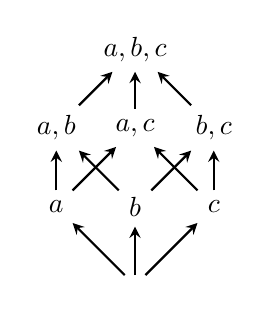
\begin{tikzpicture}[->, >=stealth, thick]
\node (1) at (2,0) {$\varnothing$};
\node (2) at (1,1) {$\set{a}$};
\node (3) at (2,1) {$\set{b}$};
\node (5) at (3,1) {$\set{c}$};
\node (6) at (1,2) {$\set{a, b}$};
\node (10) at (2,2) {$\set{a, c}$};
\node (15) at (3,2) {$\set{b, c}$};
\node (30) at (2,3) {$\set{a, b, c}$};
\draw (1) -- (2);
\draw (1) -- (3);
\draw (1) -- (5);
\draw (2) -- (6);
\draw (2) -- (10);
\draw (3) -- (6);
\draw (3) -- (15);
\draw (5) -- (10);
\draw (5) -- (15);
\draw (6) -- (30);
\draw (10) -- (30);
\draw (15) -- (30);
\end{tikzpicture}
\begin{proofitem}
\item The subsets of $S$ are represented be the powerset $\mathscr{P}(S)$.
\item Let $\mathcal{C}_\text{subset}$ be the category of subsets for a set $S$.
\item The objects $\obc{}$ of $\mathcal{C}_\text{subset}$ are the elements of
    the powerset $\mathscr{P}(S)$.
\item An arrow exists between two objects $a, b \in \mathcal{C}_\text{subset}$
    if $a\subseteq b$.
\item For $\mathcal{C}_\text{subset}$ to be a poset, it must have the following
    properties: reflexivity, transitivity, and anti-symmetry.
\setcounter{equation}{0}
\begin{align}
    A \in \mathscr{P}(S) \implies A\subseteq A &&\text{reflexivity}\\
    A,B \in \mathscr{P}(S), A\subseteq B \land B \subseteq A \implies A=B  &&\text{antisymmetry}\\
    A,B,C \in \mathscr{P}(S), A \subseteq B \land B \subseteq C \implies A
    \subseteq C&&\text{transitivity}
\end{align}
\item Thus we have shown that $\mathcal{C}_\text{subset}$ is a poset.
\end{proofitem}

\section{Small Mathematical Structures}
\subsection{Monoids}
\begin{definition}
    A category is called discrete if it has no arrows except identity arrows.
\end{definition}
In this way, categories are generalizations of sets.
\begin{definition}
    A category with only one object is called a monoid.
\end{definition}
\begin{definition}
    A monoid is a set $M$ equipped with an identity $1$ and a unital and associative
binary operation $\circ$. The monoid is sometimes written fully as $(M, \circ,
1)$.
\end{definition}
\begin{align*}
    \forall m \in& M, 1\circ m = m = m \circ 1&&\text{unital}\\
    \forall a, b, c \in& M, (a\circ b)\circ c = a \circ (b \circ
    c)&&\text{associative}
\end{align*}

\begin{ttta}
Translate between the set-theory definition of monoid and the category theory
definition of monoid.
\end{ttta}
\begin{proofitem}
    \item Let $M$ be a set of monoidal elements.
    \item Let $\mathcal{C}_\text{M}$ be a monoid category.
    \item For each $m\in M$, there is a corresponding arrow $a\in
        \mathcal{C}_\text{M}$.
    \item The set $M$ has a binary closed operation $\circ$.
    \item $M$ is equippied with an identity element $1\in M$, such that for
        $\forall m \in M, m\circ 1 = m = 1 \circ m$. This binary operation
        corresponds to the identity arrow $1_m$ in $\mathcal{C}_\text{M}$. For
        all arrows $a\in\mathcal{C}_\text{M}$, pre or post-composing $a$ with
        $1$ will yield $a$, thus proving the identity arrow for all arrows $a$.
    \item Because $\circ$ is associative in $M$, then $\forall x, y, z \in M,
        (x\circ y)\circ z = x\circ(y\circ z)$. Correspondingly, for all $a, b, c\in
        \mathcal{C}_\text{M}$ the morphism $\circ$ will associate such that
        $(a\circ b)\circ c= a\circ(b\circ c)$.
\end{proofitem}
\begin{table}
    \centering
    \begin{tabular}{ c|ccc }
    \hline
    & Set Theory & & Category Theory \\ \hline
    & & & "dummy" object \\
    Data & objects & $\rightarrow$ & arrows \\ \hline
    & identity object & $\rightarrow$ & identity arrow \\
    Structure & binary operation & $\rightarrow$ & composition \\ \hline
    & unitality & $\rightarrow$ & unitality \\
    Properties & associativity& $\rightarrow$ & associativity
    \\\hline
    \end{tabular}
    \caption{Monoid in set theory v. category theory}
\end{table}
\begin{ttta}
Can you fill in the following composition table for the arrows of this category?
Does the resulting pattern remind you of anything we’ve seen in earlier
chapters?

See Table \ref{tbl:cayley}.
\begin{table}
\centering
\begin{tabular}{c|cccc}
 $\circ$ & $1$ & $f$ & $f^2$ & $f^3$ \\
 \hline
 $1$ & $1$ & $f$ & $f^2$ & $f^3$ \\
 $f$ & $f$ & $f^2$ & $f^3$ & $1$ \\
 $f^2$ & $f^2$ & $f^3$ & $1$ & $f^2$ \\
 $f^3$ & $f^3$ & $1$ & $f^2$ & $f^2$ \\
\end{tabular}
\caption{Cayley Table}
\label{tbl:cayley}
\end{table}
\end{ttta}
\stepcounter{tttacounter}
\begin{ttta}
Find an inverse for each element of $\mathbb{Z}_4$ under addition. So for each $a \in
\mathbb{Z}_4$, find $b \in \mathbb{Z}_4$ such that $a + b \equiv 0 (\mod 4)$.
(The condition for b + a follows by commutativity.) The elements here are 0, 1,
2, 3. What about $\mathbb{Z}_n$ in general?
\end{ttta}
\begin{proofitem}
\item To find the inverse of some $a\in\mathbb{Z}_4$, we must find the
    $b\in\mathbb{Z}_4$ such that $a+b\equiv\bmod 4$.
\item One way to do this for a small $\mathbb{Z}_n$ is with a cayley table.
\item By looking at the addition cayley table for $\mathbb{Z}_4$, we can see that
    \setcounter{equation}{0}
    \begin{align}
        0+0=&0+0=0\\
        1+3=&3+1=0\\
        2+2=&2+2=0
    \end{align}
    In general, for any $\mathbb{Z}_n$, the inverse of some $a\in\mathbb{Z}_n$
    is $n-a$, such that $n-a+a=0$.
\begin{table}
\centering
\begin{tabular}{c|cccc}
 $\circ$ & $0$ & $1$ & $2$ & $3$ \\
 \hline
 $0$ & $0$ & $1$ & $2$ & $3$ \\
 $1$ & $1$ & $2$ & $3$ & $0$ \\
 $2$ & $2$ & $3$ & $0$ & $2$ \\
 $3$ & $3$ & $0$ & $2$ & $2$ \\
\end{tabular}
\caption{Cayley table for $\mathbb{Z}_4$}
\end{table}
\end{proofitem}

\subsection{Groups}
\begin{definition}
A group is a monoid in which every element has an inverse.
\end{definition}

\begin{ttta}
Produce the non-categorical definition of a group.
\end{ttta}
A group is a monoid where every element has an inverse. Therefore a group has
monoidal properties unitality and associavitity, and the additional inverse
property.
\begin{align*}
    \forall m \in& M, 1\circ m = m = m \circ 1&&\text{unital}\\
    \forall a, b, c \in& M, (a\circ b)\circ c = a \circ (b \circ c)&&\text{associative}\\
    \forall a\in& M \exists B,  a\circ b = 1 &&\text{inverse}
\end{align*}

\begin{ttta}
Can you organize this into data, structure and properties, and then see
how the structure corresponds to the properties for an equivalence relation?
\end{ttta}
See Table \ref{tbl:group}.
\begin{table}
    \centering
    \begin{tabular}{ c|ccc }
    \hline
    & Set Theory & & Category Theory \\ \hline
    & & & "dummy" object \\
    Data & objects & $\rightarrow$ & arrows \\ \hline
    & identity object & $\rightarrow$ & identity arrow \\
    & binary operation & $\rightarrow$ & composition \\
    Structure & inverse object & $\rightarrow$ & inverse arrow \\ \hline
    & unitality & $\rightarrow$ & unitality \\
    Properties & associativity& $\rightarrow$ & associativity
    \\\hline
    \end{tabular}
    \caption{Group in set theory v. category theory}
    \label{tbl:group}
\end{table}
\begin{ttta}
Try filling in these multiplication tables, in the context of the integers
mod 8 and the integers mod 10:
The numbers $1, 3, 5, 7\in \mathbb{Z}_8$, see Table \ref{tbl:z8}.
The numbers $1, 3, 7, 9\in \mathbb{Z}_{10}$, see Table \ref{tbl:z10}.
\end{ttta}
\begin{table}
\centering
\begin{tabular}{c|cccc}
 $\times $ & $1$ & $3$ & $5$ & $7$ \\
 \hline
 $1$ & $1$ & $3$ & $5$ & $7$ \\
 $3$ & $3$ & $1$ & $7$ & $5$ \\
 $5$ & $5$ & $7$ & $1$ & $3$ \\
 $7$ & $7$ & $5$ & $3$ & $1$ \\
\end{tabular}
\caption{$\mathbb{Z}_8$}
\label{tbl:z8}
\end{table}
\begin{table}
\centering
\begin{tabular}{c|cccc}
 $\times $ & $1$ & $3$ & $7$ & $9$ \\
 \hline
 $1$ & $1$ & $3$ & $7$ & $9$ \\
 $3$ & $3$ & $9$ & $1$ & $7$ \\
 $7$ & $7$ & $1$ & $9$ & $3$ \\
 $9$ & $9$ & $7$ & $3$ & $1$ \\
\end{tabular}
\caption{$\mathbb{Z}_{10}$}
\label{tbl:z10}
\end{table}

\begin{ttta}
Can you make a definition of a group directly as a category satisfying some conditions?
\end{ttta}
A group extends a monoid, so let's start with the definition of the monoidal
category---a category where there is only object. From there we must add the
concept of an inverse, so we'll say that for every arrow in $a \in \mathcal{C}$
there exists an arrow $b\in\mathcal{C}| a\cdot b = b\cdot a = 1_a$.

\section{Set and Functions}
\subsection{Underlying importance}
Sets are the starting point for structures such as posets, monoids, topological
spaces and groups. Depending on the structure in question, the set is imbued
with some additional property---an ordering, a binary operation, or a notion of
closeness.
\begin{quote}
	The starting point for the maps between structures is the concept of a
	function---the basic notion of a map between sets.
\end{quote}
We then find a good notion of map between special structures by
looking at maps that preserve the special properties in question.
\begin{definition}
	Let $f, g$ be functions $A\rightarrow B$. We say $f = g$ as functions whenever
	$\forall a \in A, f(a) = g(a)$.
\end{definition}
\begin{ttta}
	How many different functions are possible between 3 inputs and 2 outputs? What
	if there were p inputs and k outputs?
	\begin{align*}
		2^3 &  & \text{3 inputs, 2 outputs} \\
		k^p &  & \text{p inputs, k outputs} \\
	\end{align*}
\end{ttta}
\begin{ttta}
	How many different functions are possible between $0$ inputs and $n$ outputs.
	How many different functions are possible between $n$ inputs and $0$ outputs.
	Can you interpret it?
	\begin{align*}
		n^0 & =1 &  & \text{input }\varnothing  \\
		0^n & =1 &  & \text{output }\varnothing \\
	\end{align*}
	The way to interpret this is that when $\varnothing$ is the output set, there is
	only one function from $n$ inputs.  Each input of $n$ is mapped to $\varnothing$
	like $n_i \mapsto \varnothing$. When the input is $\varnothing$ we get an absurd
	situation where one must produce an element of the $\varnothing$ to get an output.
	There is only way to produce such an absurdity.
\end{ttta}
\begin{ttta}
	\begin{enumerate}[label = {(\alph*)}]
		\item Show that sets and functions form a category.
		\item Check that the identity really behaves like an identity, both on
		      the left and on the right.
		\item Check that composition is
		      associative.\label{ttta:function-forms-category}
	\end{enumerate}
\end{ttta}
To form a category, there are two required properties: unitality and
associativity. Consider the category \textbf{Set} where sets are objects and
functions are arrows.
\begin{align*}
	(1_b \circ f)(x)                    & = 1_b(f(x))        &  &                       \\
	                                    & = f(x)             &  & \text{left identity}  \\
	(f \circ 1_a)(x)                    & = f(1_b(x))        &  &                       \\
	                                    & = f(x)             &  & \text{right identity} \\
	\left((f \circ g) \circ h\right)(x) & = (f \circ g)h(x)  &  & \text{}               \\
	                                    & = f(g(h(x)))       &  & \text{}               \\
	\left(f \circ (g \circ h)\right)(x) & = f((g\circ h)(x))                            \\
	                                    & = f(g(h(x)))       &  & \text{associativity}
\end{align*}

\section{Large worlds of mathematical structures}
\subsection{Monoids and Homomorphisms}
Suppose some function $f: \mathbb{N} \rightarrow \mathbb{Z}$ and $f(n)=n$. This function
$f$ respects addition in the following sense.
\begin{align*}
    f(m+n) = f(m) + f(n)
\end{align*}
We can add $m+n$ first and then map it via $f$, or we can first map $m, n$ via
$f$, and then add them.

\begin{ttta}
Another possible function $f: \mathbb{N} \rightarrow \mathbb{Z}$ is given by
$f(n) = 2n$. See if you can check that this also satisfies the above condition
$f(m+n) = f(m) + f(n)$.
\begin{align*}
    f(m+n) =& f(m) + f(n)\\
    2(m+n) =& 2(m) + 2(n)\\
    2(m+n) =& 2(m+n)\\
    m+n =& m+n
\end{align*}
Thus we have shown that $f$ respects addition.
\end{ttta}

\begin{ttta}
Show that this function
\[
f=\set{(0, 0), (1, 1), (2, -1), (3, 2), (4, -2), (5, 3), (6, -3), \dots}
\]
does not respect addition.
\begin{align*}
    f(1+3) =& f(1) + f(3)\\
    f(4) =& f(1) + f(3)\\
    -2 =& 1 + 2\\
    -2 \neq& 3
\end{align*}
\end{ttta}

\begin{ttta}
Mapping into the integers is special because it turns out that respecting
addition forces a function to respect the identity. Prove it.
\end{ttta}
\begin{proofitem}
\item To respect addition a function $f$ must satisfy the following equation $f(m+n) =
f(m)+f(n)$.  Let us suppose that $f$ does respect addition and show that it
implies that $f$ also respects the identity.
\begin{align*}
    f(0+n) =& f(0) + f(n)\\
    f(n) =& f(0) + f(n)\\
    f(0) =& 0
\end{align*}
\end{proofitem}
\begin{definition}
Let $A$ and $B$ be monoids, and write the identity as $1$ and the
binary operation as $\circ$ in each case. Then a monoid homomorphism from A to
B is a function $f:A\rightarrow B$ on the underlying sets, such that
\begin{align*}
    \forall x, y \in A, f(x \circ y) &= f(x) \circ f(y)&&f\text{ respects }\circ\\
    f(1)&=1&&f\text{ respects identity}
\end{align*}
\end{definition}

\stepcounter{tttacounter}
\begin{ttta}
What do we need to check to show that monoids and their homomorphisms form a
category?
\end{ttta}
\begin{proofitem}
\item Let $M$ be the set of monoids, $M_A, M_B, M_C, \ldots, \in M$.
\item Let $\mathcal{C}_\text{mon}$ be a category where each object is a monoid
    $A\in M$, and each arrow $\times$ is a mapping $A,B \in M, \times:
    A\rightarrow B$.
\item Let $f, g$ be composable functions, ie they are arrows between objects.
\item Let $\circ$ be a binary composition operation on arrows.
\item Let $\ast$ be a binary composition operation on monoidal elements.
\item To show that monoids and their homomorphisms form a cateogry we must show
    the properties of unitality and associativity.
\setcounter{equation}{0}
\begin{align}
    (g\circ f)(x\ast y) &= g(f(x\ast y)) && \text{def. of }\circ\\
    &= g(f(x) \ast f(y)) && f\text{ respects }\ast\\
    &= g(f(x)) \ast g(f(y)) && g\text{ respects }\ast\\
    &= (g\circ f)(x) \ast (g\circ f)(y) && \text{def. of }\circ\\
    (g\circ f)(1)&= g(f(1)) && \text{def. of }\circ\\
    &= g(1) && f \text{ respects }1\\
    &= 1 && g \text{ respects }1
\end{align}
\end{proofitem}
\begin{figure}[H]
\documentclass[border=0.2cm]{standalone}
\usepackage{tikz}
\usepackage{titlesec}
\usepackage{float}
\usepackage{standalone}
\usepackage{tikzit}
\usetikzlibrary{automata, arrows.meta, positioning}
\usetikzlibrary{arrows.meta, positioning}
\input{figures/sample-02.tikzstyles}

\begin{document}
\begin{tikzpicture}[scale=1.0]
	\begin{pgfonlayer}{nodelayer}
		\node [style=object] (0) at (0, 0) {$M_A$};
		\node [style=object] (1) at (4, 0) {$M_B$};
		\node [style=object] (2) at (8, 0) {$M_C$};
	\end{pgfonlayer}
	\begin{pgfonlayer}{edgelayer}
		\path [-stealth, thick]
		(0) edge node[above] {$f$}   (1)
		(1) edge node[above] {$g$}   (2)
		(0) edge [out=210, in=240, looseness=8, below]  node {$x$}(0)
		(0) edge [out=330, in=300, looseness=8, below]  node {$y$}(0)
		(0) edge [loop above] node[above] {$x\ast y$}(0)
		(1) edge [out=210, in=240, looseness=8, below]  node {$x$}(1)
		(1) edge [out=330, in=300, looseness=8, below]  node {$y$}(1)
		(1) edge [loop above] node[above] {$f(x\ast y)$}(1)
		(2) edge [out=210, in=240, looseness=8, below]  node {$x$}(2)
		(2) edge [out=330, in=300, looseness=8, below]  node {$y$}(2)
		(2) edge [loop above] node[above] {$(g\circ f)(x\ast y)$}(2) ;
	\end{pgfonlayer}
\end{tikzpicture}
\end{document}

\caption{Monoid Category $\mathbf{Monoid}$}
\end{figure}
\subsection{Groups}
\begin{ttta}
Define group homomorphism as a function respecting the group structure. When
dealing with groups, it is redundant to ask for the identity to be preserved.
It’s also redundant to ask for the inverses to be preserved. Prove this.
\end{ttta}
\begin{proofitem}
\item The properties needed for a group are identity, inverse, and
    associativity. We can show that if there exists a function $f$ which is a
    group homomorphism, then we get inverse and identity for freebeez.
\item Suppose $f: G \rightarrow H$ is a homomorphism between groups $G$ and $H$. Then:
\begin{align*}
    f(x\ast x^{-1}) &= f(1_G)\\
    f(x)\ast f(x^{-1}) &= 1_H
\end{align*}
\item Therefore $f(x^{-1})$ is indeed the inverse of $f(x)$ and inverse is
    preserved.
\begin{align*}
    f(x\ast 1_G) &= f(x)\\
    f(x)\ast f(1_G) &= f(x)\\
    f(x^{-1})\ast f(x)\ast 1_H &= f(x^{-1})\ast f(x)\\
    1_H &= f(x^{-1}\ast x)\\
    1_H &= f(1_G)
\end{align*}
\item Therefore identity is preserved.
\end{proofitem}

\begin{ttta}
Do we have to check anything else to show that groups and group homomorphisms form a category?
\end{ttta}
Because groups are monoids with an extra property, there is nothing to check
because monoids already form a cateogry. In other words, the monoidal nature of
a group is sufficient to show unitality and associativity for a category created
from some set that is also a group.

\subsection{Posets}
\begin{ttta}
Create a definition of an order-preserving function for posets in general by
analogy with the structure-preserving maps we've seen already.
\end{ttta}
\begin{proofitem}
\item Let $f:P\rightarrow Q$ be some function between two posets $P$ and $Q$.
    Because $P$ and $Q$ are posets, we know that individually they both have the
    properties reflexivity, transitivity, and antisymmetry. For $f$ to be order
    preserving, the only condition on $f$ is
\begin{align*}
    x\geq_P y \implies f(x)\geq_Q f(y)
\end{align*}
\end{proofitem}

\begin{ttta}
Do we have to check anything to show that we have a category of posets and order-preserving functions?
\end{ttta}
\begin{proofitem}
    \item To check that we have a category, we must assure unitality and
        associativity are preserved.
\end{proofitem}
\begin{align*}
    x \geq y &\implies f(x) \geq f(y) \\
             &\implies g(f(x) \geq g(f(y)) \\
             &\implies (g\circ f)(x) \geq (g\circ f)(y) \\
\end{align*}
\begin{figure}[H]
    \begin{center}
\documentclass[border=0.2cm]{standalone}
\usepackage{tikz}
\usepackage{titlesec}
\usepackage{float}
\usepackage{standalone}
\usepackage{tikzit}
\usetikzlibrary{automata, arrows.meta, positioning}
\usetikzlibrary{arrows.meta, positioning}
\input{sample-02.tikzstyles}

\begin{document}
\begin{tikzpicture}
	\begin{pgfonlayer}{nodelayer}
		\node [style=object] (0) at (0, 0) {$P_A$};
		\node [style=object] (1) at (4.5, 0) {$P_B$};
		\node [style=object] (2) at (9, 0) {$P_C$};
	\end{pgfonlayer}
	\begin{pgfonlayer}{edgelayer}
        \path [-stealth, thick]
        (0) edge node[above] {$f$}   (1)
        (1) edge node[above] {$g$}   (2)
        (0) edge [out=30, in=60, looseness=8, below]  node[above] {$1$}(0)
        (0) edge [out=120, in=150, looseness=8, below] node[above] {$x\ast y$}(0)
        (0) edge [out=210, in=240, looseness=8, below]  node[below] {$x$}(0)
        (0) edge [out=300, in=330, looseness=8, below]  node[below] {$y$}(0)
        (1) edge [out=30, in=60, looseness=8, below]  node[above] {$f(1)$}(1)
        (1) edge [out=120, in=150, looseness=8, below] node[above] {$f(x\ast y$)}(1)
        (1) edge [out=210, in=240, looseness=8, below]  node[below] {$f(x)$}(1)
        (1) edge [out=300, in=330, looseness=8, below]  node[below] {$f(y)$}(1)
        (2) edge [out=30, in=60, looseness=8, below]  node[above, xshift=1cm] {$(g\circ f)(1)$}(2)
        (2) edge [out=120, in=150, looseness=8, below] node[xshift=-0.4cm,above] {$(g\circ f)(x\ast y$)}(2)
        (2) edge [out=210, in=240, looseness=8, below]  node[xshift=-0.5cm, below] {$(g\circ f)(x)$}(2)
        (2) edge [out=300, in=330, looseness=8, below]  node[xshift=0.5cm, below] {$(g\circ f)(y)$}(2)
        ;
	\end{pgfonlayer}
\end{tikzpicture}
\end{document}

\end{center}
\caption{Poset Category $\mathbf{Poset}$}
\end{figure}

\begin{ttta}
Think again about the poset of factors of 42.
Observe that $6 < 7$ but 6 is higher than 7 in this diagram. What two orderings
are we considering on the same set of numbers here, and what map is it that is
not order-preserving?
\end{ttta}
\begin{figure}[H]
    \begin{center}
        \input{42-factor}
    \end{center}
    \caption{42-factor lattice}
\end{figure}
\begin{proofitem}
\item Let $S=\set{1,2, 3, 6, 7, 14, 21, 42}\subset \mathbb{N}$.
\item One order is $\geq$ as defined on $\mathbb{N}$.
    The other order is divides $\mid$, as in $a\mid b$---for example $6\mid 12$.
    Both orders are reflexive, anti-symmetric, and transitive, as required by
    definition.
\item Let us consider the map $f:\mathbb{N}\rightarrow\mathbb{N}$, where $f=+1$.
    For the ordering $\geq$, $f$ preserves ordering.
\begin{align*}
    f(x \geq y) =& f(x) \geq f(y)\\
        =& x+1 \geq y+1\\
        =& x \geq y
\end{align*}
Now we will show that $f$ does not preserve ordering on $\mid$ by
counter-example.
\begin{align*}
    f(x \mid y) =& f(x) \mid f(y)&&\text{Let }x=7, y=14\\
    f(7 \mid 14) =& f(7) \mid f(14)\\
     \neq& 8 \mid 15
\end{align*}
Thus we have shown that $\mid$ does not preserve ordering.
\end{proofitem}

\subsection{Categories}
\begin{ttta}
Think of a sensible starting point for a definition of a morphism of
categories $F: \mathbb{C} \longrightarrow \mathbb{D}$. It should map objects to
objects and arrows to arrows, but if we start with an arrow $x \xrightarrow{f}
y\in\mathbb{C}$ what should the source and target of $F(f)$ be in
$\mathbb{D}$?
\end{ttta}
\begin{proofitem}
    \item
    \begin{align*}
        f\in \mathbb{C}&: x \rightarrow y\\
        F(f)\in \mathbb{D}&: F(x) \rightarrow F(y)
    \end{align*}
\end{proofitem}

\begin{ttta}
Come up with the definition of a morphism between categories, starting
with the action of $F$ on objects and arrows. Then proceeding by making
sure it is structure-preserving. To do this, you need to be clear what the
structure of a category is: identities and composition. Once you've done this,
can you check that this gives us a category of small categories and all
morphisms between them.
\end{ttta}

% \include{02set theory}
% \include{03kleisli}
% \include{04products and coproducts}

% \backmatter
% \printbibliography
\end{document}
